\documentclass[main.tex]{subfile}
\begin{document}

\section{Delopgave 2\\\normalsize{-- Multitrådet FIFO buffer som kædet liste.}}
Denne delopgave har til formål at vise, at vi har forståelse for hvordan hægtedelister fungere samt hvordan disse kan implementeres i C. Udover at demonsterer vores forståelse for hægtedelister tjener opgaven det formål at demonstrer hvordan nogle af risiciene ved flertrådet systemer kan forebygges.

\subsection{Implementationen, overordnet set}
Implementationen af vores løsning til denne delopgave begrænser sig til klassen \texttt{list.c}. I forbindelse med test af vores implementation har vi også ændret filen \texttt{main.c}, hvor vi har introduceret to nye funktioner \texttt{test()} og \texttt{add(void *param)}. Vi vil beskrive implementationen af disse funktioner samt deres formål i afsnit~\ref{sec:del2_test} på side~\pageref{sec:del2_test}.\\

I \texttt{list.c} kan vores implementation splittes i tre dele.
\begin{enumerate}
\item Tilføjelse af elementer til listen. Implementationen af denne funktionalitet begrænser sig til funktionen \texttt{list\_add(List *l, Node *n)} og har til formål at hægte det nye elemt \texttt{n} bagerst på listen.
\item Fjernelse af elementer fra listen. Implementationen af denne funktionalitet begrænser sig til funktionen \texttt{list\_remove(List *l)} og har til formål at fjerne og returnere de foreste element i den hægtede liste.
\item Trådsikring af listen, ved hjælp af gensidig udelukkelse. I modsætning til de to foregående dele er denne del spredt over flere af implementationens funktioner. Dette skyldes at mutexen skal oprettes sammen med listen, men låses og frigives i forbindelse med metodekald.  
\end{enumerate}

\subsection{De specifikke løsninger}
\subsubsection{Tilføjelse af elementer}
For at tilføje et element til en liste skal vi bruge en pointer til både listen og til det element som skal hægtes på listen. Når et element tilføjes til en liste hægtes dette på listens bagerste element således at de ældste elementer altid ligger tættest på listens start. I vores implementation ændre vi listens bagerste element således at det peger på det nye element. Her efter undersøger vi om den knude der tilføjes til listen indgår i en sekvens af hægtede knuder. Er dette tilfældet traversere vi listen af knuder igennem indtil vi når det sidste element. Når vi har nået det sidste element ændre vi den hægtede listes \texttt{last} pointer således at denne nu også peger på det nye slut element. Herefter opdatere vi listens længde med antallet af nye elementer. 

\subsubsection{Fjernelse af elementer}
Ved fjernelse af elementer starter vi med at gennem den hægtede listes \texttt{rod} element til en variabel for at simplificere arbejds processen. Da roden ikke må fjernes tjekker vi om \texttt{next} pointeren på roden peger på en værdi. Er dette tilfældet ændres rodens \texttt{next} pointer så den perger på det element der ligger efter elementet der skal fjernes, hvorefter længden reduceres med en og det fjernede element retuneres. Peger rodens \texttt{next} pointer ikke på en værdi er listen tom og værdien \texttt{NULL} returneres.

\subsubsection{Trådsiking}
For at introducere trådsikring til vores program har vi gjort brugt af en binær semafor, bedre kendt som en \texttt{mutex}. Mutexen har til formål at sikre at kun en tråd kan eksekver en given kommando ad gangen. Dette fungere ved at den tråd der kun den tråd der i en given situation har låst mutexen kan eksekvere den efterfølgende kode, mens andre tråder der ønsker at eksekver den samme kode, eller eksekver anden kode, som også er beskyttet af mutexen, bliver holdt tilbage indtil låsen på mutexen fjernes og en ny tråd kan låse den.\\

I vores implementation har vi gjort brug af én mutex som bliver brugt både når tråde ønsker at tilføje eller fjerne et element fra listen. Det gør sig gældende for både \texttt{list\_add} og \texttt{list\_remove} funktionen at når en tråd træder ind i funktionen skal den låse mutexen før end at den får lov at tilføje eller fjerne noget, og tilsvarende frigive mutexen når operationen er udført. Dette betyder at hvis en anden tråd er i gang med at redigere listen, må tråden vente på at mutexen bliver frigivet før den kan udføre sine ændringer på listen.\\

Mutexen bliver oprette sammen med listen og ødelægges sammen med listen ved brug af funktions kaldet \texttt{list\_destroy}.

\subsection{Fejl og mangler}
Selvom at vi i vores implementation gør brug at mutex til at sikre at tråde ikke tilgår listens elementer samtidigt, og at brugen af kun én mutex skulle forhindre eventuelle deadlocks i at opstå er der stadig en måde hvorpå vores system ville gå i knæ. Hvis en bruger tilføjet en sekvens af knuder som danner en løkke vil vores implementation træde ind i en uendelig løkke da den ved indsættelse af nye elementer læder efter det sidste element i rækken af elementer.\\

Vi har gjort os nogle overvejelser om hvordan denne situation kunne afværges og er fundet frem til at den bedste løsning ville være at gemme det foreste af de nye elementer til en varialbel og så tjekke at ingen af de efterfælgende elementer peger tilbage på dette element. Denne løsning til sikre at en liste hvor bagerste element tilbage på det forreste ville blive opdaget, men samtidig udelukker det ikke situationer hvor fx bagerste element peger tilbage på det anded element i listen. Den enestå måde hvorpå vi har kunnet se at det er muligt at afvære en sådan situation, hvor et element peger tilbage på et tidligere, er ved at gemme alle nye elementer til variabler og sikre at ingen af disse bliver peget på senere i listen. Vi har valgt ikke at givet os i kast med at implementere en sådan løsning da det ikke virker til at være opgavens primære mål, men det er bestemt en situation der er værd at overveje hvis programmet skal anvendes i større stil.\\

En anden ting som fangede vores opmærksomhed under implementationen af denne opgave var muligheden for at gøre brug af 2 mutex objekter. Så længer at den hægtede liste ikke er tom der er i og forsig ikke noget i vejen for at en process tilføjer et element mens en anden fjerner et element da de arbejder på hver sin del af listen og derfor ikke skal bruge de samme objekter. Den eneste situation hvor dette ikke er tilfældet er hvis listen er tom eller kun holder et element, da begge porcesser i såfald ville arbejde på listens rod og derved risikere at forsage en race-condition. En tilgang til dette kunne være kun at låse \texttt{list\_add} og \texttt{list\_remove} enkeltvis så længe at listen holder to eller flere elementer, men låse begge funktioner hvis listen er tom eller kun holder et element.

\subsection{Test}\label{sec:del2_test}
For at teste at vores implementation kan anvendes af flertrådet programmer har vi skrevet en test funktion i \texttt{main.c}. Funktionene opretter to tråde som begge har tilopgave tilføje ti elementer til listen. For at sikre at begge tråde forsøger at tilgå listen samtidig har til tilføjet et kald til funktionen \texttt{sleep(1)} som får den aktueller tråd til at sove i et sekund.\\

For at kontrollere at trådene ikke har overskrevet hinandens ændringer afsluttes funktionen med at printe alle elementerne i den hægtede liste til terminalen. Af figur~\ref{fig:opg2_2_test} ses det at alle 20 elementer er blivet tilføjet til listen, og at tråedene på skift har haft adgang til listen. 

\begin{figure}[H]
\center
\fbox{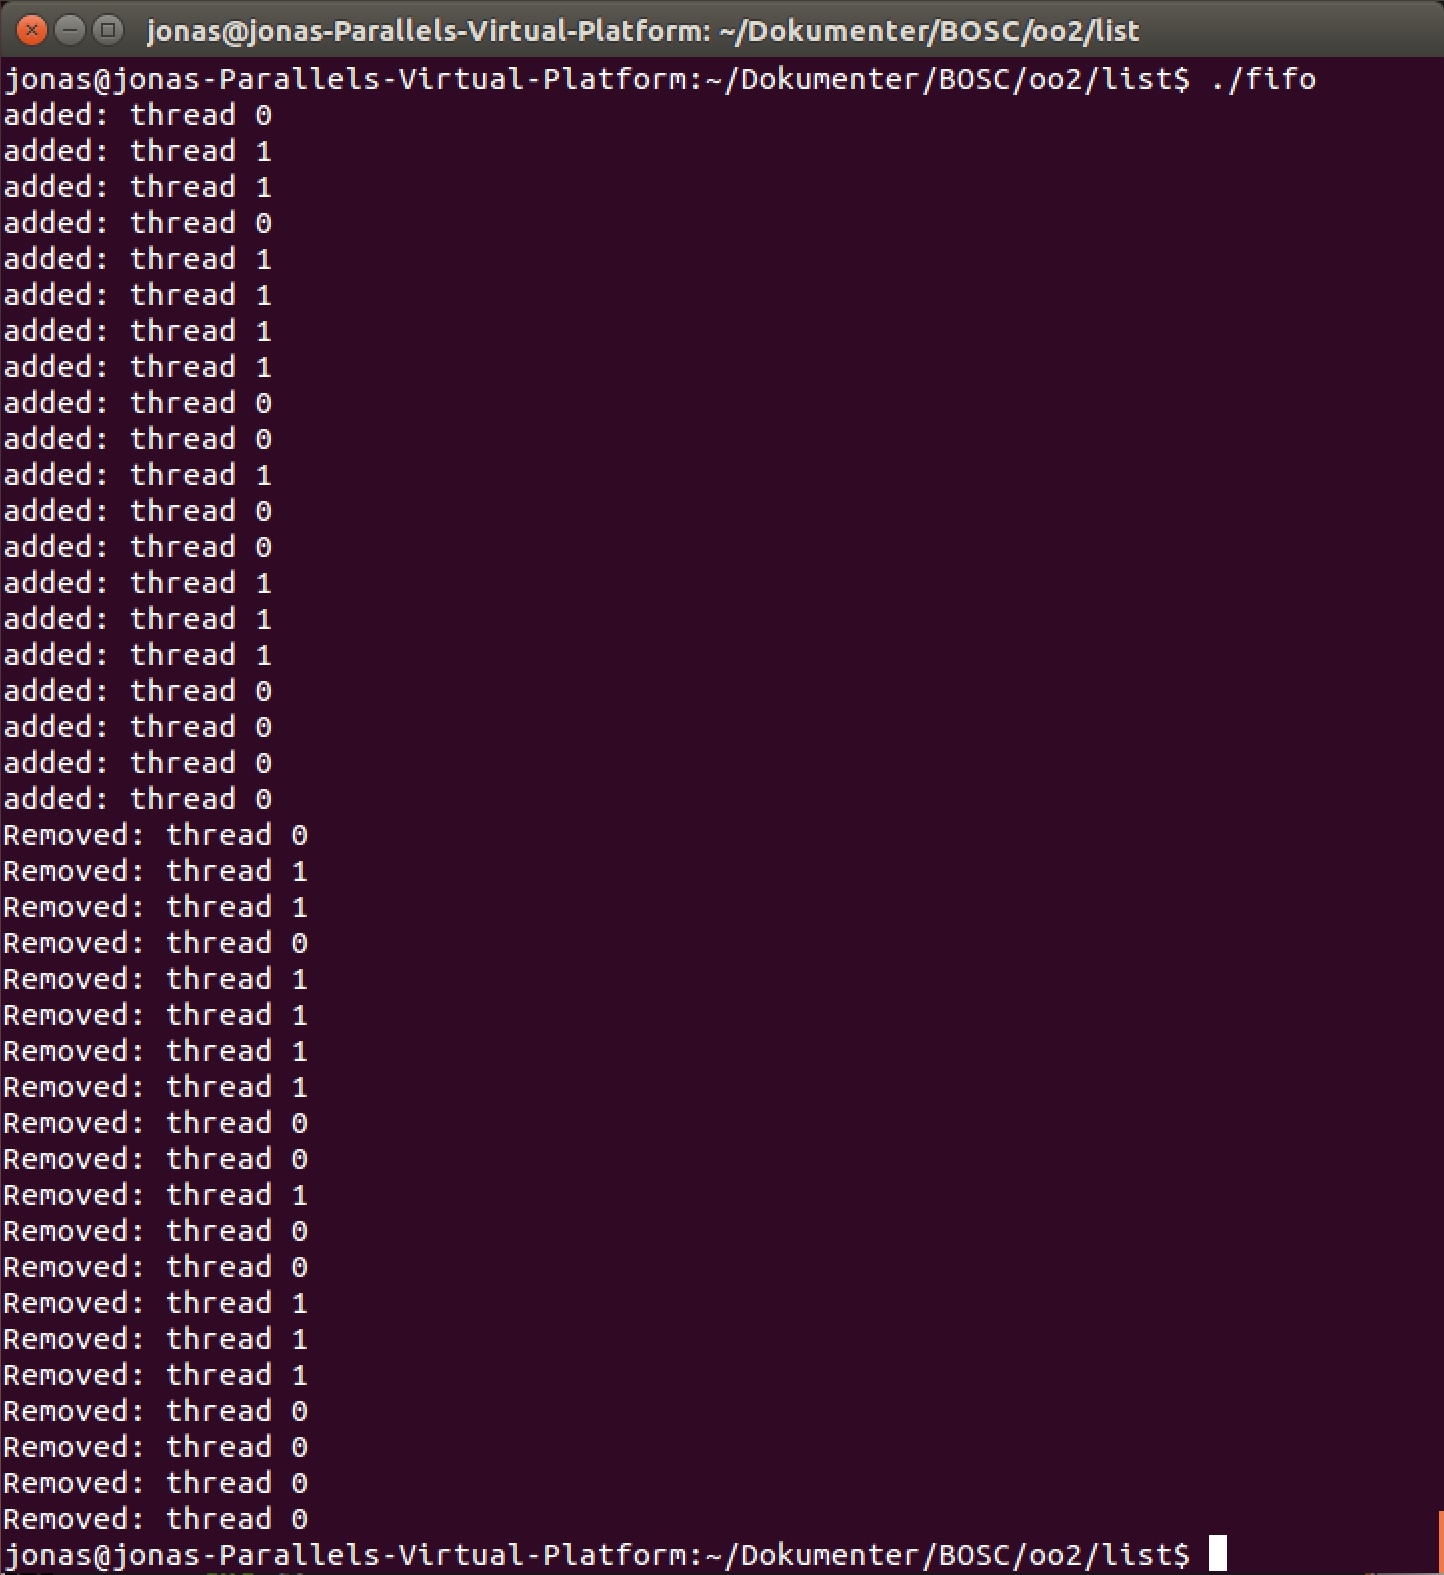
\includegraphics[width=0.85\textwidth]{test_opg_2_2.png}}
\caption{Udskrift at test resultat til terminalen.}
\label{fig:opg2_2_test}
\end{figure}

\subsubsection{En anden tilgang til test}
En anden mulig måde at teste hvorvidt vores hægtedeliste understøtter at flere tråde forsøger at tilgå den er ved brugen af funktionskaldet \texttt{pthread\_mutex\_trylock()} som returnere en fejlmeddelelse hvis den givne mutex allerede låst. På denne måde kan man få de enkelte tråde til at printe en besked til terminalen når de er tvunget til at vente på at låsen på mutexen bliver frigivet. 
\end{document}